\section{\RU{Текстовые строки}\EN{Text strings}}

\subsection{\CCpp}

\label{C_strings}
\RU{Обычные строки в Си заканчиваются нулем}\EN{The normal C strings are zero-terminated} 
(\ac{ASCIIZ}-\RU{строки}\EN{strings}).

\RU{Причина, почему формат строки в Си именно такой (оканчивающийся нулем) вероятно историческая}
\EN{The reason why the C string format is as it is (zero-terminated) is apparently historical}.
\RU{В}\EN{In} \cite{Ritchie79} \RU{мы можем прочитать}\EN{we read}:

\begin{framed}
\begin{quotation}
A minor difference was that the unit of I/O was the word, not the byte, because the PDP-7 was a word-addressed
machine. In practice this meant merely that all programs dealing with character streams ignored null
characters, because null was used to pad a file to an even number of characters.
\end{quotation}
\end{framed}

\index{Hiew}
\RU{Строки выглядят в Hiew или FAR Manager точно так же}
\EN{In Hiew or FAR Manager these strings looks like this}:

\begin{lstlisting}
int main()
{
	printf ("Hello, world!\n");
};
\end{lstlisting}

\begin{figure}[H]
\centering
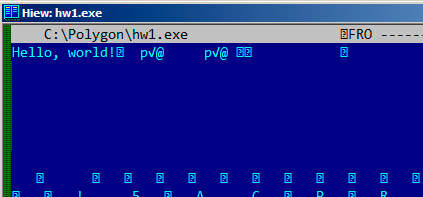
\includegraphics[scale=\NormalScale]{digging_into_code/strings/C-string.png}
\caption{Hiew}
\end{figure}

\subsection{Borland Delphi}
\index{Pascal}
\index{Borland Delphi}
\RU{Когда кодируются строки в Pascal и Delphi, 
сама строка предваряется 8-битным или 32-битным значением,
в котором закодирована длина строки.}
\EN{The string in Pascal and Borland Delphi is preceded by an 8-bit or 32-bit string length.}

\RU{Например}\EN{For example}:

\begin{lstlisting}[caption=Delphi]
CODE:00518AC8                 dd 19h
CODE:00518ACC aLoading___Plea db 'Loading... , please wait.',0

...

CODE:00518AFC                 dd 10h
CODE:00518B00 aPreparingRun__ db 'Preparing run...',0
\end{lstlisting}

\subsection{Unicode}

\index{Unicode}
\RU{Нередко уникодом называют все способы передачи символов, когда символ занимает 2 байта или 16 бит}
\EN{Often, what is called Unicode is a methods for encoding strings where each character occupies 2 bytes or 16 bits}.
\RU{Это распространенная терминологическая ошибка}\EN{This is a common terminological mistake}.
\RU{Уникод --- это стандарт, присваивающий номер каждому символу многих письменностей мира, но не описывающий
способ кодирования}\EN{Unicode is a standard for assigning a number to each character in the many writing systems of the 
world, but does not describe the encoding method}.

\index{UTF-8}
\index{UTF-16LE}
\RU{Наиболее популярные способы кодирования}\EN{The most popular encoding methods are}: 
UTF-8 (\RU{наиболее часто используется в Интернете и *NIX-системах}\EN{is widespread in Internet and *NIX systems})
\AndENRU UTF-16LE (\RU{используется в}\EN{is used in} Windows).

\subsubsection{UTF-8}

\index{UTF-8}
UTF-8 \RU{это один из очень удачных способов кодирования символов}\EN{is one of the most successful methods for
encoding characters}.
\RU{Все символы латиницы кодируются так же, как и в ASCII-кодировке, а символы, выходящие за пределы
ASCII-7-таблицы, кодируются несколькими байтами}\EN{All Latin symbols are encoded just like in ASCII,
and the symbols beyond the ASCII table are encoded using several bytes}.
\RU{$0$ кодируется, как и прежде, нулевыми байтом, так что все стандартные
функции Си продолжают работать с UTF-8-строками так же как и с обычными строками}\EN{$0$ is encoded as
before, so all standard C string functions work with UTF-8 strings just like any other string}.

\RU{Посмотрим, как символы из разных языков кодируются в UTF-8 и как это выглядит в FAR, в кодировке 437}
\EN{Let's see how the symbols in various languages are encoded in UTF-8 and how it looks like in FAR, using the 437 codepage}
\footnote{\RU{Я взял пример и переводы на разные языки здесь}\EN{I've got the example and translations from here}: 
\url{http://go.yurichev.com/17304}}:

\begin{figure}[H]
\centering
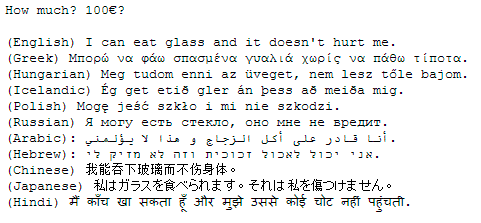
\includegraphics[scale=\NormalScale]{digging_into_code/strings/multilang_sampler.png}
\end{figure}

\begin{figure}[H]
\centering
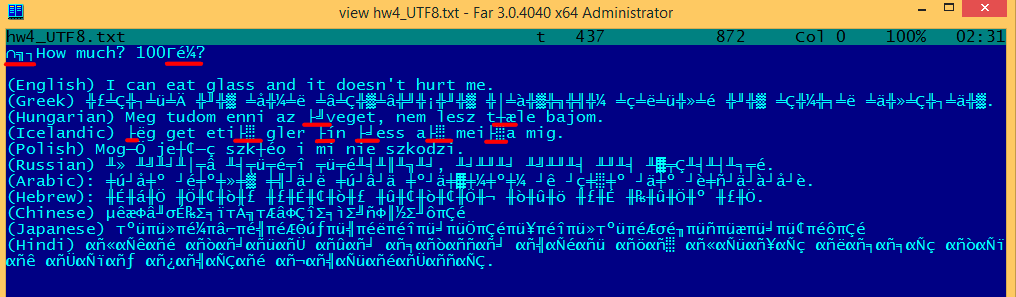
\includegraphics[scale=\FigScale]{digging_into_code/strings/multilang_sampler_UTF8.png}
\caption{FAR: UTF-8}
\end{figure}

\RU{Видно, что строка на английском языке выглядит точно так же, как и в ASCII-кодировке}
\EN{As you can see, the English language string looks the same as it is in ASCII}.
\RU{В венгерском языке используются латиница плюс латинские буквы с диакритическими знаками}
\EN{The Hungarian language uses some Latin symbols plus symbols with diacritic marks}.
\RU{Здесь видно, что эти буквы кодируются несколькими байтами, я подчеркнул их красным}
\EN{These symbols are encoded using several bytes, I underscored them with red}.
\RU{То же самое с исландским и польским языками}\EN{It's the same story with the Icelandic and Polish languages}.
\RU{В самом начале я также применил символ валюты ``Евро'', который кодируется тремя байтами}
\EN{I also used the ``Euro'' currency symbol at the start, which is encoded with 3 bytes}.
\RU{Остальные системы письма здесь никак не связаны с латиницей}
\EN{The rest of the writing systems here have no connection with Latin}.
\RU{По крайней мере о русском, арабском, иврите и хинди мы можем сказать, что здесь видны повторяющиеся
байты, что не удивительно, ведь, обычно буквы из одной и той же системы письменности расположены в одной
или нескольких таблицах уникода, поэтому часто их коды начинаются с одних и тех же цифр}
\EN{At least in Russian, Arabic, Hebrew and Hindi we can see some recurring bytes, and that is not surprise:
all symbols from a writing system are usually located in the same Unicode table, so their code begins with
the same numbers}.

\RU{В самом начале, перед строкой ``How much?'', видны три байта, которые на самом деле \ac{BOM}}
\EN{At the beginning, before the ``How much?'' string we see 3 bytes, which are in fact the \ac{BOM}}.
\EN{The }\ac{BOM} \RU{показывает, какой способ кодирования будет сейчас использоваться}\EN{defines the encoding system to be
used}.

\subsubsection{UTF-16LE}

\index{UTF-16LE}
\index{Windows!Win32}
\RU{Многие функции win32 в Windows имееют суффикс}\EN{Many win32 functions in Windows have the suffixes} \TT{-A} 
\AndENRU \TT{-W}.
\RU{Первые функции работают с обычными строками, вторые с UTF-16LE-строками}\EN{The first type of functions works
with normal strings, the other with UTF-16LE strings} (\IT{wide}).
\RU{Во втором случае, каждый символ обычно хранится в 16-битной переменной типа \IT{short}}
\EN{In the second case, each symbol is usually stored in a 16-bit value of type \IT{short}}.

\RU{Cтроки с латинскими буквами выглядят в Hiew или FAR как перемежающиеся с нулевыми байтами}
\EN{The Latin symbols in UTF-16 strings look in Hiew or FAR like they are interleaved with zero byte}:

\begin{lstlisting}
int wmain()
{
	wprintf (L"Hello, world!\n");
};
\end{lstlisting}

\begin{figure}[H]
\centering
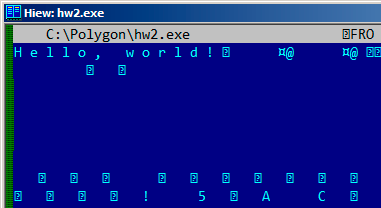
\includegraphics[scale=\NormalScale]{digging_into_code/strings/UTF16-string.png}
\caption{Hiew}
\end{figure}

\RU{Подобное можно часто увидеть в системных файлах \gls{Windows NT}}\EN{We can see this often in \gls{Windows NT} 
system files}:

\begin{figure}[H]
\centering
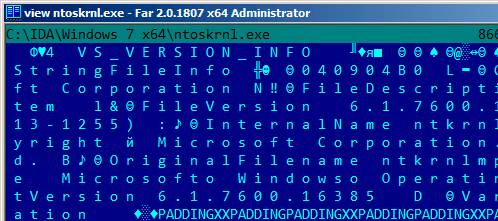
\includegraphics[scale=\NormalScale]{digging_into_code/strings/ntoskrnl_UTF16.png}
\caption{Hiew}
\end{figure}

\index{IDA}
\RU{В \IDA, уникодом называется именно строки с символами, занимающими 2 байта}\EN{Strings with characters
that occupy exactly 2 bytes are called ``Unicode'' in \IDA}:

\begin{lstlisting}
.data:0040E000 aHelloWorld:
.data:0040E000                 unicode 0, <Hello, world!>
.data:0040E000                 dw 0Ah, 0
\end{lstlisting}

\RU{Вот как может выглядеть строка на русском языке}\EN{Here is how the Russian language 
string}\RU{ (``И снова здравствуйте!'')} \RU{закодированная в UTF-16LE}\EN{is encoded in UTF-16LE}:

\begin{figure}[H]
\centering
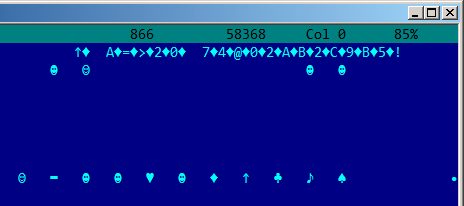
\includegraphics[scale=\NormalScale]{digging_into_code/strings/russian_UTF16.png}
\caption{Hiew: UTF-16LE}
\end{figure}

\RU{То что бросается в глаза --- это то что символы перемежаются ромбиками (который имеет код 4)}
\EN{What we can easily spot is that the symbols are interleaved by the diamond character (which has the ASCII code of 4)}.
\RU{Действительно, в уникоде кирилличные символы находятся в четвертом блоке}\EN{Indeed, the Cyrillic symbols
are located in the fourth Unicode plane}
\footnote{\href{http://go.yurichev.com/17003}{wikipedia}}.
\RU{Таким образом, все кирилличные символы в UTF-16LE находятся в диапазоне}\EN{Hence, all
Cyrillic symbols in UTF-16LE are located in the} \TT{0x400-0x4FF}\EN{ range}.

\RU{Вернемся к примеру, где одна и та же строка написана разными языками}\EN{Let's go back to the example with the
string written in multiple languages}.
\RU{Здесь посмотрим в кодировке UTF-16LE}\EN{Here is how it looks like in UTF-16LE}.

\begin{figure}[H]
\centering
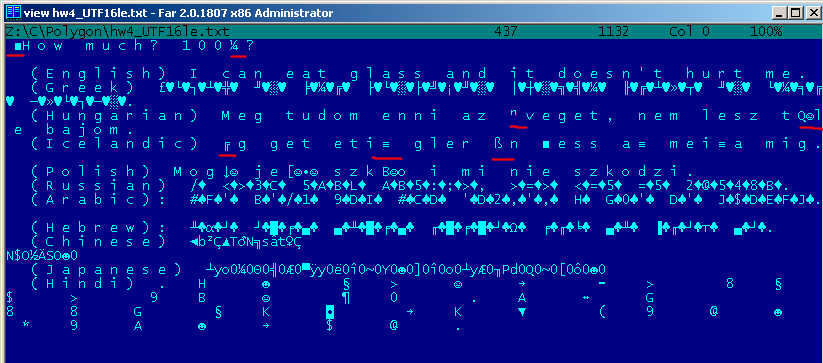
\includegraphics[scale=\FigScale]{digging_into_code/strings/multilang_sampler_UTF16.png}
\caption{FAR: UTF-16LE}
\end{figure}

\RU{Здесь мы также видим \ac{BOM} в самом начале}\EN{Here we can also see the \ac{BOM} in the beginning}.
\RU{Все латинские буквы перемежаются с нулевыми байтом}\EN{All Latin characters are interleaved with a zero byte}.
\RU{Некоторые буквы с диакритическими знаками (венгерский и исландский языки) также подчеркнуты красным}
\EN{I also underscored in red some characters with diacritic marks (Hungarian and Icelandic languages)}.

% TODO: strings *NIX utility. procmonitor also shows strings...

\subsection{Base64}
\index{Base64}

\RU{Кодировка base64 очень популярна в тех случаях, когда нужно передать двоичные данные как текстовую строку.}
\EN{The base64 encoding is highly popular for the cases when you need to transfer binary data as a text string.}
\RU{По сути, этот алгоритм кодирует 3 двоичных байта в 4 печатаемых символа:}
\EN{In essence, this algorithm encodes 3 binary bytes into 4 printable characters:}
\RU{все 26 букв латинского алфавита (в обоих регистрах), цифры, знак плюса (``+'') и слэша (``/''),}
\EN{all 26 Latin letters (both lower and upper case), digits, plus sign (``+'') and slash sign (``/''),}
\RU{в итоге это получается 64 символа}\EN{64 characters in total}.

\RU{Одна отличительная особенность строк в формате base64, это то что они часто (хотя и не всегда) заканчиваются
одним или двумя символами знака равенства (``='') для выравнивания, например:}
\EN{One distinctive feature of base64 strings is that they often (but not always) end with 1 or 2 padding 
equality symbol(s) (``=''), for example:}

\begin{lstlisting}
AVjbbVSVfcUMu1xvjaMgjNtueRwBbxnyJw8dpGnLW8ZW8aKG3v4Y0icuQT+qEJAp9lAOuWs=
\end{lstlisting}

\begin{lstlisting}
WVjbbVSVfcUMu1xvjaMgjNtueRwBbxnyJw8dpGnLW8ZW8aKG3v4Y0icuQT+qEJAp9lAOuQ==
\end{lstlisting}

\RU{Так что знак равенства (``='') никогда не встречается в середине строк закодированных в base64.}
\EN{The equality sign (``='') is never encounter in the middle of base64-encoded strings.}
